\documentclass[hide notes,intlimits]{beamer}

\mode<presentation>
{
  \usetheme[footline]{UAFshadealert}
  \setbeamercovered{transparent}
}

% frames are 128 millimeters by 96 millimeters

% load packages
\usepackage[english]{babel}
\usepackage[latin1]{inputenc}
\usepackage[T1]{fontenc}
\usepackage{amsmath,amssymb,wasysym}
\usepackage{lmodern}

\usepackage{tikz}
\usetikzlibrary{shapes,arrows,shadows}

\usepackage{empheq}
\usepackage{color}
\usepackage{animate}

\graphicspath{{../figs/}}

% Some useful commands (from MPL)
\newcommand{\s}[1]{\ensuremath{\,\text{#1}}}
\newcommand{\unit}[1]{\ensuremath{\,\text{#1}}}

\definecolor{dark red}{HTML}{E41A1C}
\definecolor{dark green}{HTML}{4DAF4A}
\definecolor{dark violet}{HTML}{984EA3}
\definecolor{dark blue}{HTML}{084594}
\definecolor{dark orange}{HTML}{FF7F00}
\definecolor{light blue}{HTML}{377EB8}
\definecolor{light red}{HTML}{FB9A99}
\definecolor{light violet}{HTML}{CAB2D6}

\setbeamercolor{boxed}{fg=black,bg=uaf yellow}


\newenvironment{transbox}{%
  
\begin{tikzpicture}
    \node[drop shadow,rounded corners,text width=\textwidth,fill=white, fill opacity=0.6,text opacity=1] \bgroup
  }{
    \egroup;\end{tikzpicture}} 

\newenvironment{transbox-tight}{%
  \begin{tikzpicture}
    \node[drop shadow,rounded corners,fill=uaf yellow, fill opacity=0.75,text opacity=1] \bgroup
  }{
    \egroup;\end{tikzpicture}} 


% title page
\title[Better subglacial hydrology into PISM]{Better subglacial hydrology into \\ the Parallel Ice Sheet Model}
\subtitle{a work in progress}

\author[Bueler \and van Pelt]{Ed Bueler\inst{*} and Ward van Pelt\inst{\dagger}}
\institute{\inst{*} University of Alaska Fairbanks \and %
           \inst{\dagger} IMAU, Utrecht, Netherlands}

\date{IGS June 2012}


\begin{document}

\setbeamertemplate{background canvas}
{
  % empty
}

% insert titlepage
\begin{frame}
  \titlepage
\end{frame}


\newcommand{\scream}[1]{\alert{\textbf{#1}}}

\begin{frame}
  \frametitle{PISM = Parallel Ice Sheet Model}

  \begin{center}
      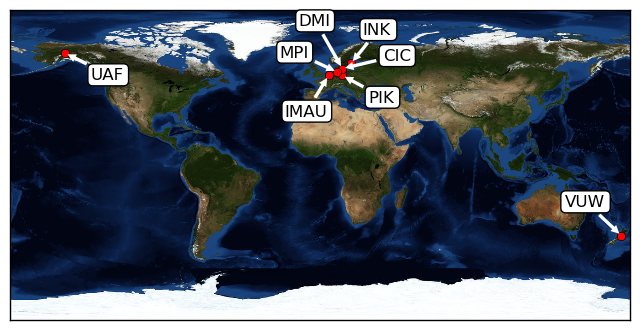
\includegraphics[width=80mm]{pism-users-map}
  \end{center}

\vspace{-2mm}
  \begin{itemize}
  \item \alert{\large\texttt{www.pism-docs.org}}  and  \url{help@pism-docs.org}
  \item runs on laptops to supercomputers
  \item documented releases once a year
  \item \emph{User's Manual} with real modeling examples including Greenland Ice Sheet, Ross Ice Shelf, and St\"orglaciaren
  
  \bigskip
  \scriptsize
  \item[$\circ$] supported by the NASA Modeling, Analysis and Prediction
  \item[$\circ$] jointly developed by UAF and Potsdam Inst.~for Climate Impact Research
  \end{itemize}
\end{frame}


\newcommand{\whytitle}{why we need better subglacial hydrology}

\begin{frame}
  \frametitle{\whytitle}
  \framesubtitle{motivation 1}

\vspace{-6mm}
\begin{center}
  we are \scream{NOT} conserving mass (of liquid water)
\end{center}

\vspace{-5mm}
\begin{columns}
\begin{column}{0.5\textwidth}
  \begin{itemize}
    \item current basal hydrology in PISM has an independent ``can'' of porous till at each location
      \begin{itemize}
        \item[$\ast$] ``can'' receives basal melt
        \item[$\ast$] ``overflows'' at 2m of water \dots \emph{overflow lost}
        \item[$\ast$] provides till yield stress
        \item[$\ast$] suitable for Siple coast ice streams (Tulaczyk et al 2000)      \end{itemize}
    \item missing:
    
      \begin{center} \emph{lateral transport of water} \end{center}
  \end{itemize}
\end{column}
\begin{column}{0.5\textwidth}
\begin{center}
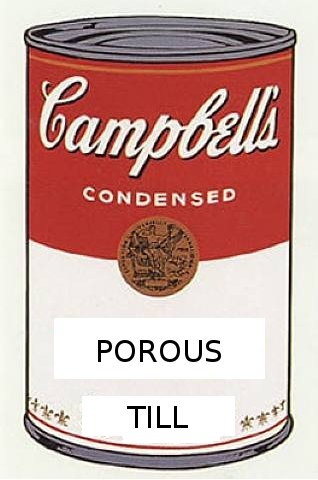
\includegraphics[height=0.3\textheight]{till-warhol-soup}

%\vspace{1mm}

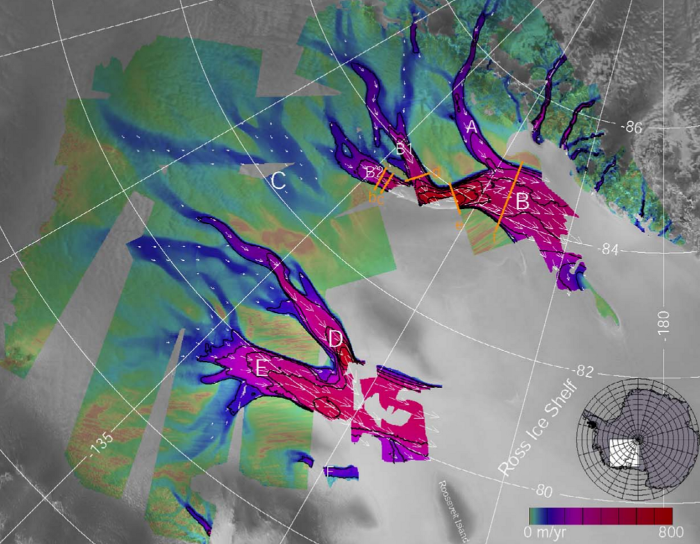
\includegraphics[height=0.45\textheight]{siple}
\end{center}
\end{column}
\end{columns}
\end{frame}


\begin{frame}
  \frametitle{\whytitle}
  \framesubtitle{motivation 2}

\vspace{-6mm}
\begin{center}
  we \scream{ARE} conserving energy (better than before)
\end{center}
  
\vspace{-2mm}
  \begin{itemize}
    \item better energy conservation using enthalpy
    \item new basal melt rate distribution ($\text{mm}\,\text{a}^{-1}$):
  \end{itemize}

  \begin{center}
    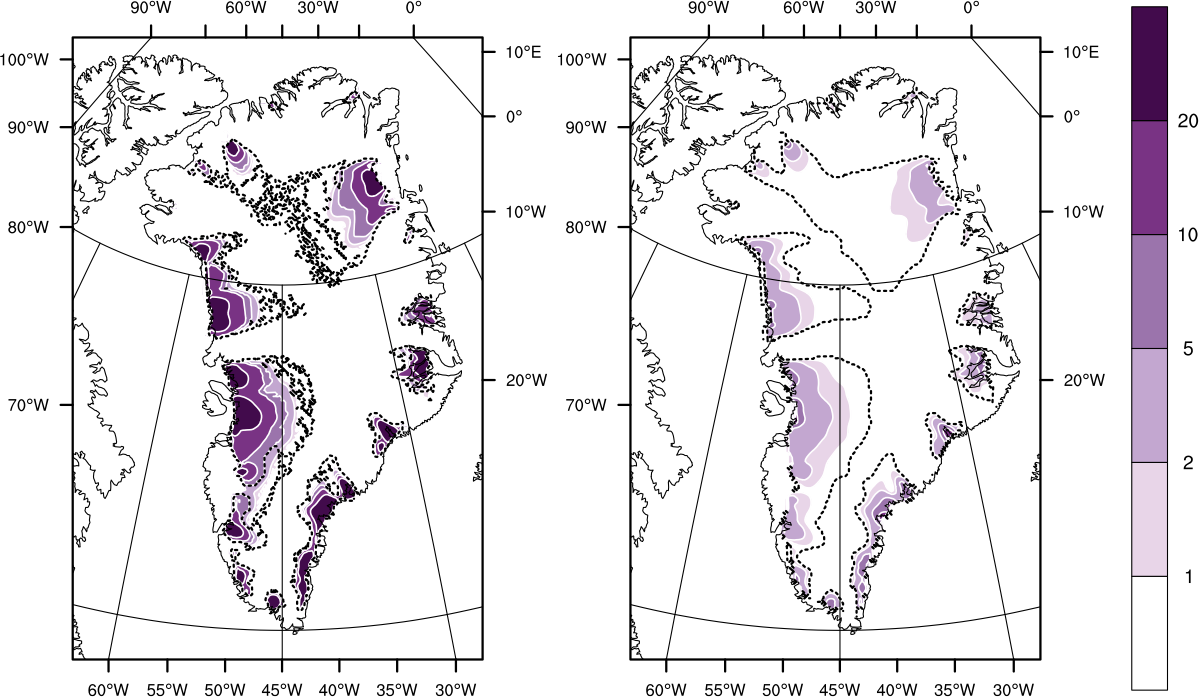
\includegraphics[height=0.57\textheight]{enthalpy-model-crop}
    
    \medskip
    \scriptsize \textbf{left}: using \underline{enthalpy} \qquad\qquad\quad \textbf{right}: using \underline{temperature}

\medskip
    \tiny Aschwanden et al (2012), \emph{An enthalpy formulation for glaciers and ice sheets}, J. Glaciol.
  \end{center}
\end{frame}


\begin{frame}
  \frametitle{example existing uses of PISM subglacial hydrology}

\begin{columns}
\begin{column}{0.5\textwidth}
\begin{center}
model locations of Antarctic ice streams without inversion

\vspace{10mm}

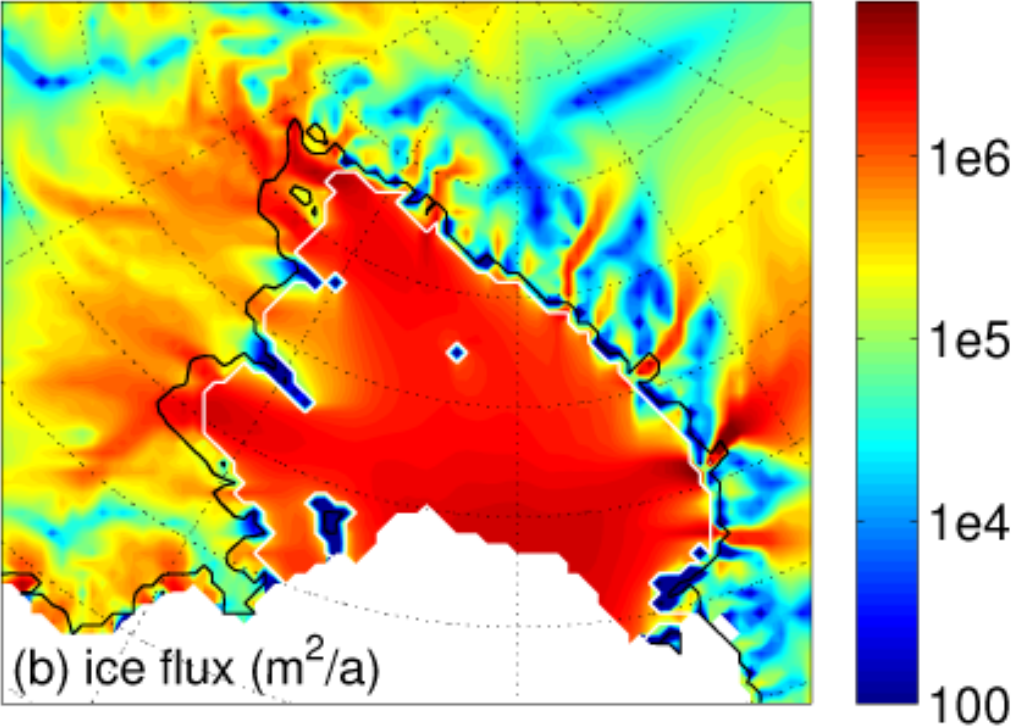
\includegraphics[width=0.9\textwidth]{martin-fig12}

\vspace{7mm}

\medskip
\scriptsize (Martin et al., 2011, \emph{The Cryosphere})
\end{center}
\end{column}
\begin{column}{0.5\textwidth}
\begin{center}
study sliding and cyclicity/surging

\bigskip
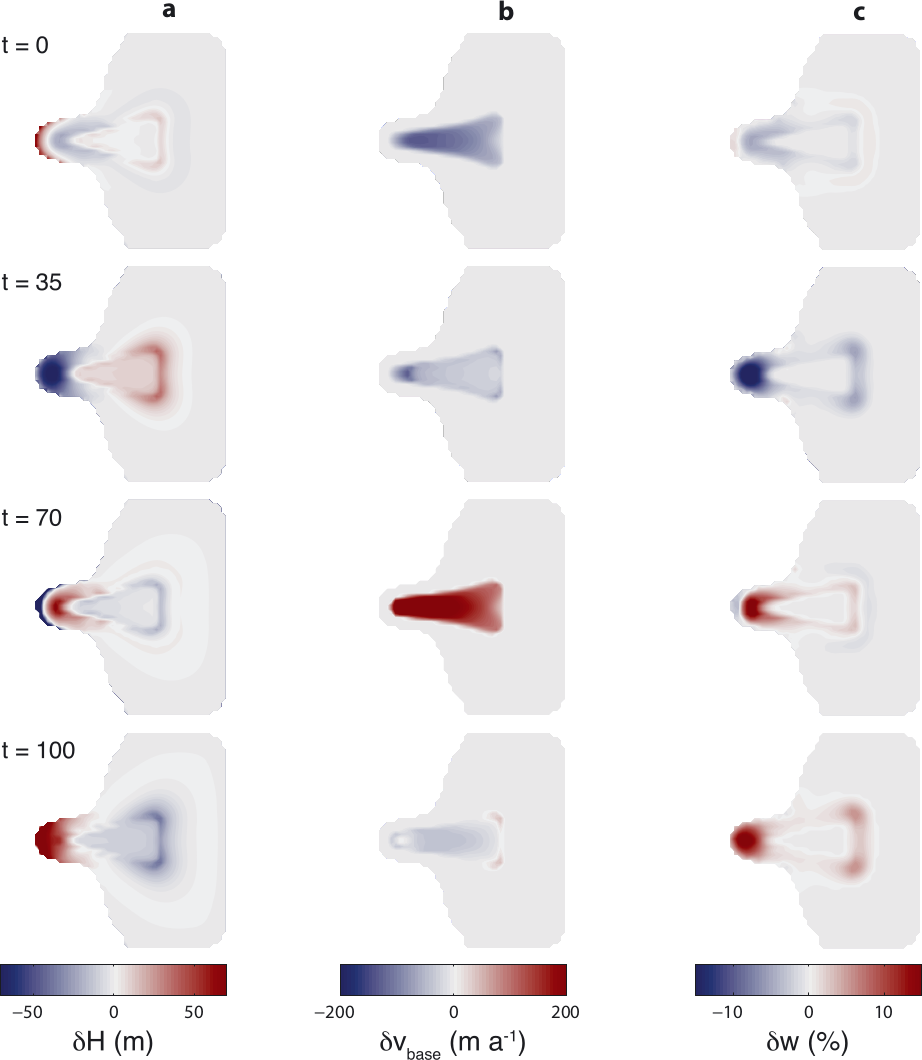
\includegraphics[width=0.8\textwidth]{vanPeltOerlemans-fig4}

\medskip
\scriptsize (van Pelt \& Oerlemans, 2012, \emph{J.~Glaciol.})
\end{center}
\end{column}
\end{columns}
\end{frame}


\begin{frame}
  \frametitle{the goal}

\begin{center}
\scream{improve PISM by adding mass-conserving subglacial hydrology}
\end{center}

\bigskip\bigskip\bigskip
subgoals:

\begin{enumerate}
  \item provide reasonable default behavior
  \item introduce minimum number of new tunable parameters
  \item provide playground for testing sliding models
\end{enumerate}

\end{frame}


\begin{frame}
  \frametitle{elements of subglacial hydrology}
  \framesubtitle{can we agree on these?}

\newcommand{\bq}{\mathbf{q}}
  \begin{itemize}
    \item \textbf{conservation of mass}:
    
    $$W_t + \nabla \cdot \bq = m / \rho_w$$

where $W=$ spatially-averaged thickness of water layer, $\bq=$ flux, $m=$ supply rate ($\text{kg}\,\text{m}^{-2}\,\text{s}^{-1}$)

    \item \textbf{hydraulic potential} {\color{blue} for top of water sheet}:
    
    $$\phi = p_w + \rho_w g (b{\color{blue} + W})$$

where $\phi=$ hydraulic potential, $b=$ bedrock elevation

    \item \textbf{some kind of Darcy flow}:
    
    $$\bq = - \frac{K W}{\rho_w g} \nabla \phi$$
    
    where $K=$ hydraulic conductivity (\emph{not} constant in general)
    
    \medskip\medskip
    \scriptsize or \quad $\bq = - k W^\alpha |\nabla \phi|^{\beta - 2} \nabla \phi$ \quad etc.

  \end{itemize}

\end{frame}


\begin{frame}
  \frametitle{elements of subglacial hydrology}
  \framesubtitle{whence pressure?}

  \begin{itemize}
    \item combine previous three equations to get one equation in two unknowns
      \begin{itemize}
      \item[$\ast$] water thickness $W$ and pressure $p_w$ are unknown
      \end{itemize}
      
    \item an \emph{closure} equation is needed to determine $p_w$
  \end{itemize}

\end{frame}


\begin{frame}
  \frametitle{closure alternatives}

  \begin{itemize}
    \item creep dominates so ice presses on water (classical?):
        $$p_w = \rho_i g H$$
      \begin{itemize}
      \vspace{-4mm}
      \item[$\ast$]  e.g.~static subglacial lake
      \item[$\ast$]  zero effective pressure
      \item[$\ast$]  \dots but we could try:  $p_w = s\, \rho_i g H$ with $0<s<1$
      \end{itemize}

\bigskip
    \item generates porous medium equation (Flowers \& Clarke 2002):
        $$p_w = \rho_i g H \left(\frac{W}{W_{\text{crit}}}\right)^\gamma$$
      \begin{itemize}
      \vspace{-1mm}
      \item[$\ast$]  where $\gamma=7/2$ and $W_{\text{crit}}=0.1$ m, for example
      \item[$\ast$]  e.g.~on Trapridge Glacier
      \end{itemize}
  \end{itemize}

\end{frame}


\begin{frame}
  \frametitle{more closure alternatives}

      \begin{itemize}
      \item physical models for opening and closure of a distributed system
        \begin{itemize}
        \item[$\ast$]  evolution equation for [$Y=$ average cavity depth] must be of the form (Hewitt, 2011)
        $$Y_t = W_O - W_C$$
          \begin{itemize}
          \vspace{-4mm}
          \item[$\circ$] $W_O$ is total from opening processes (wall melt, sliding, \dots)
          \item[$\circ$] $W_C$ is total from closing processes (ice creep, sedimentation, \dots)
          \end{itemize}
        \item[$\ast$] indirectly determines water pressure $p_w$
        \end{itemize}
      
      \bigskip
      \item but wait: there are channels, too! (R\"othlisberger 1972)

\begin{center}
\medskip
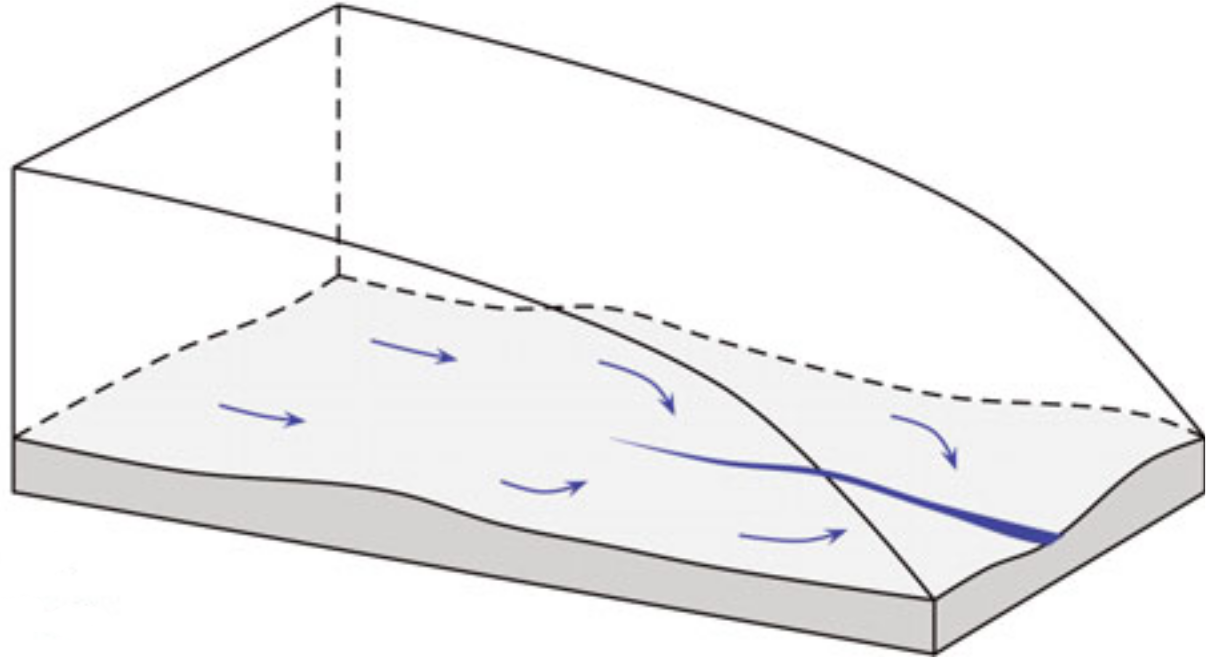
\includegraphics[width=0.4\textwidth]{hewitt-cartoon} \tiny figure from (Hewitt, 2011)
\medskip
\end{center}
    \end{itemize}
\end{frame}


\begin{frame}
  \frametitle{yet more alternatives}
  \framesubtitle{\dots from Vancouver, B.C.~area as usual}

\small
\begin{columns}
\begin{column}{0.6\textwidth}
  \begin{itemize}
  \item  Creyts \& Schoof (2009): bed protrusions stabilize sheet flow
      \begin{itemize}
      \vspace{-1mm}
      \item[$\ast$] vs Walder (1982): sheet flow unstable
      \end{itemize}

  \bigskip
  \item  Schoof (2010): fixed-location 2D network of channels
      \begin{itemize}
      \vspace{-1mm}
      \item[$\ast$] grid-refinement limit not known?
      \end{itemize}
      
  \bigskip
  \item  Hewitt \& Schoof \& Werder (2012):
      \begin{itemize}
      \vspace{-1mm}
      \item[$\ast$] water pressure bounds: $0 \le p_w \le \rho_i g H$
      \item[$\ast$] elliptic variational inequality for $p_w$
      \item[$\ast$] large areas where $p_w = \rho_i g H$ anyway?
      \end{itemize}
  \end{itemize}
\end{column}

\begin{column}{0.4\textwidth}
\begin{center}
\vspace{-5mm}
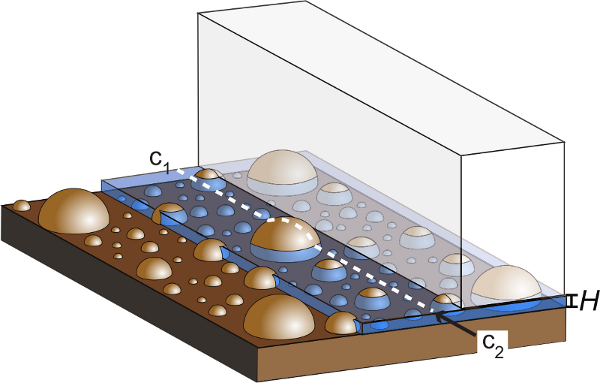
\includegraphics[width=0.85\textwidth]{creyts-sheetflow}

\vspace{4mm}

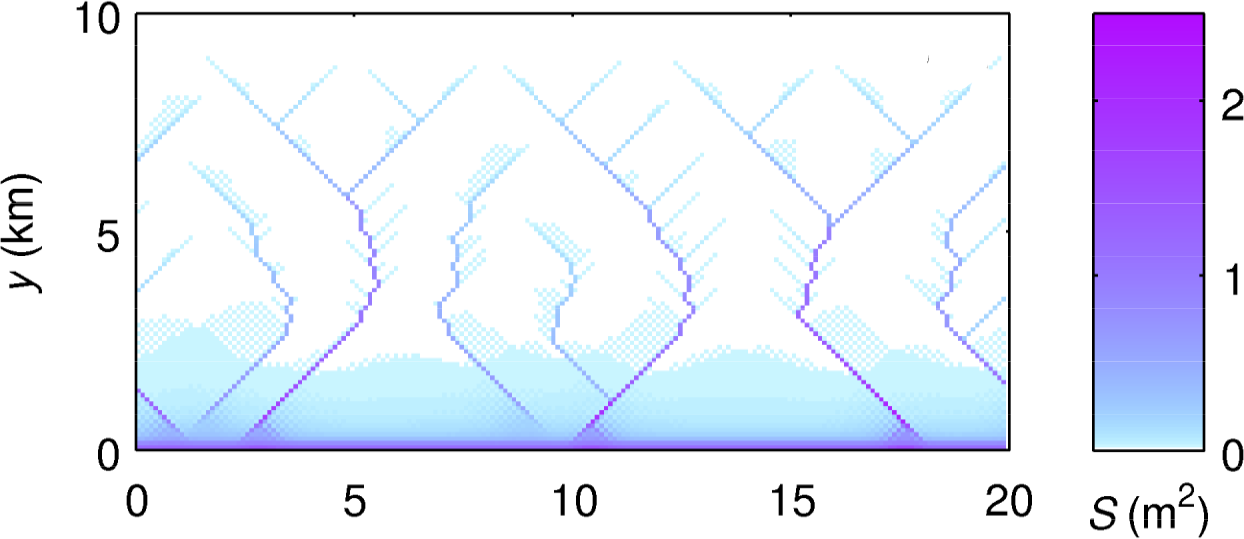
\includegraphics[width=1.0\textwidth]{schoof-channels}

\vspace{5mm}

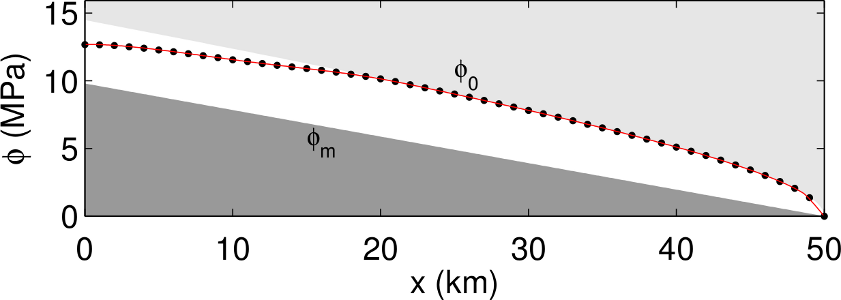
\includegraphics[width=1.0\textwidth]{schoof-overburden}
\end{center}
\end{column}
\end{columns}

\end{frame}


\begin{frame}
  \frametitle{too many tunable parameters!}

  \begin{itemize}
  \item we hope to explore above possibilities in PISM
  \item but it has finally dawned on us:
  
  \begin{center}
  \emph{exploring processes through modeling is different from improving default behavior for ice sheet simulation}
  \end{center}
  \end{itemize}
\end{frame}


\begin{frame}
  \frametitle{back to something basic}

  \begin{itemize}
    \item recall the simple model where creep dominates:
    		$$p_w = \rho_i g H$$
    \item hydraulic potential:
      $$\phi = \rho_i g H + \rho_w g (b+W) = \rho_i g \,h + (\rho_w - \rho_i) g \,b + \rho_w g \,W$$
    \item combining all equations gives:
       $$\boxed{W_t + \nabla\cdot\left(\mathbf{v} W\right) = \nabla \cdot(K W \nabla W) + m / \rho_w}$$
      \begin{itemize}
      \vspace{-3mm}
      \item[$\ast$] $\mathbf{v} = - K \left[r \nabla h + (1-r) \nabla b\right]$  \quad where $r = \rho_i/\rho_w$
      \item[$\ast$] an advection-diffusion equation
      \end{itemize}
  \end{itemize}
\end{frame}


\begin{frame}
  \frametitle{velocity and time scales in the ``basic'' model}

  \begin{itemize}
    \item velocity from spatial gradients of elevations:
      $$\mathbf{v} = - K \Big[r \nabla h + (1-r) \nabla b\Big]$$
    \item what happens with real data (\emph{ALBMAPv1}) for $h(x,y)$ and $b(x,y)$?
    \begin{center}
    \medskip
     \qquad 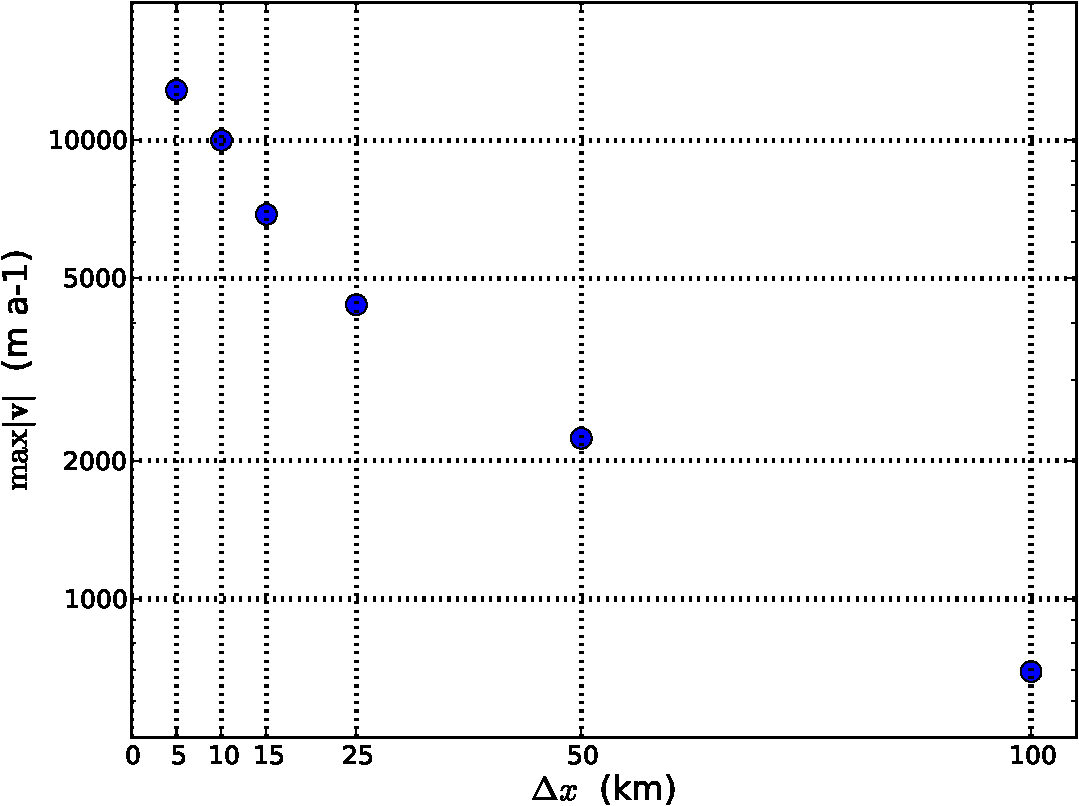
\includegraphics[width=0.4\textwidth]{vresults}
    \medskip
    \end{center}
       \small
       \begin{itemize}
       \item[$\ast$] may need a regularization (smoothing or cap) on $\mathbf{v}$
       \end{itemize}
       \normalsize
    \item diffusivity $D = K W$ small but $K$ uncertain \dots another regularization?
  \end{itemize}

\end{frame}


\begin{frame}
  \frametitle{toy Antarctic Ice Sheet example}

\vspace{-5mm}
  \begin{itemize}
  \small
    \item toy \emph{Matlab} results: uniform $1 \,\,\text{cm}\,\text{a}^{-1}$ melt rate, 20ka run
    
      \begin{center}
      %\medskip
      \includegraphics<1>[width=0.5\textwidth]{water_20ka_100km}
      \includegraphics<2>[width=0.5\textwidth]{water_20ka_50km}
      \includegraphics<3>[width=0.5\textwidth]{water_20ka_25km}
      \end{center}

       \small
       \begin{itemize}
       \item[$\ast$] far too much water (PISM run would give mostly frozen bed \dots)
       \item[$\ast$] convergence under grid refinement evident (100km, 50km, 25km)
       \end{itemize}
       \normalsize
  \item Johnson (2002) studied distribution of subglacial lakes with related model
  \end{itemize}

\end{frame}


\begin{frame}
  \frametitle{practical benefit with the basic model}
 
\begin{itemize}
\item  \scream{report the amount of subglacial water delivered at each outlet}
\item \dots as we can already report the amount of ice delivered at an outlet, through automatic identification of ``drainage basins''
  \begin{itemize}
  \item[$\ast$] e.g.~Jakobshavn basins below
  \end{itemize}
\end{itemize}

\vspace{-5mm}

\begin{columns}
\begin{column}{0.5\textwidth}
\begin{center}
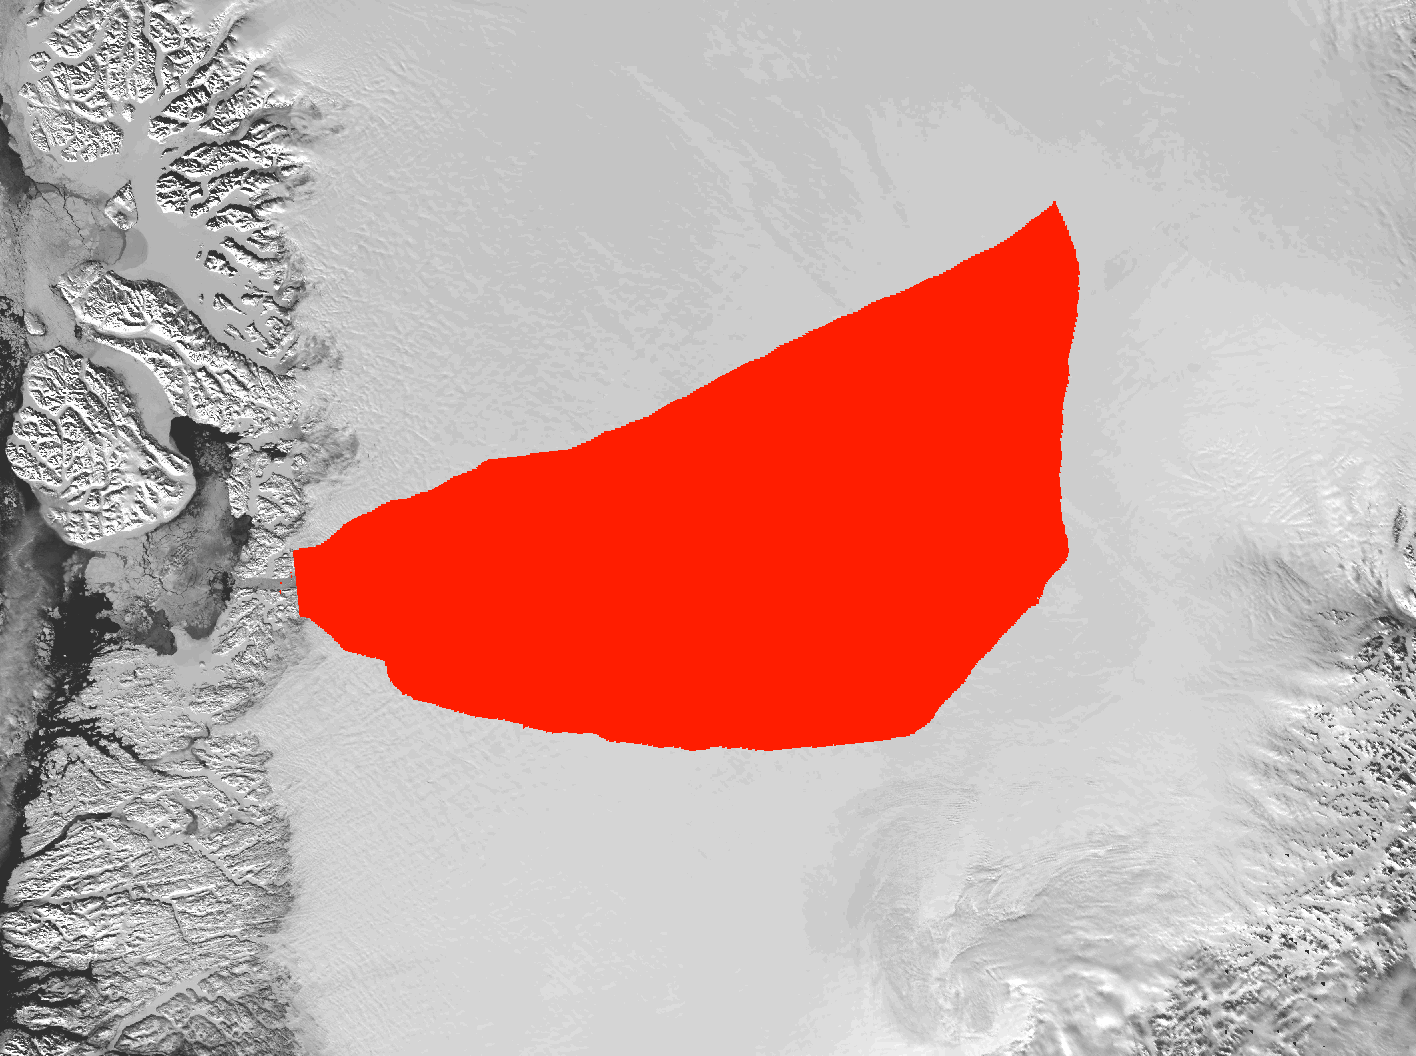
\includegraphics[width=0.85\textwidth]{ftt-mask}

basin for $-\nabla h$ flow,

\phantom{where $\phi$}

for ice
\end{center}
\end{column}
\begin{column}{0.5\textwidth}
\begin{center}
\vspace{0.5mm}

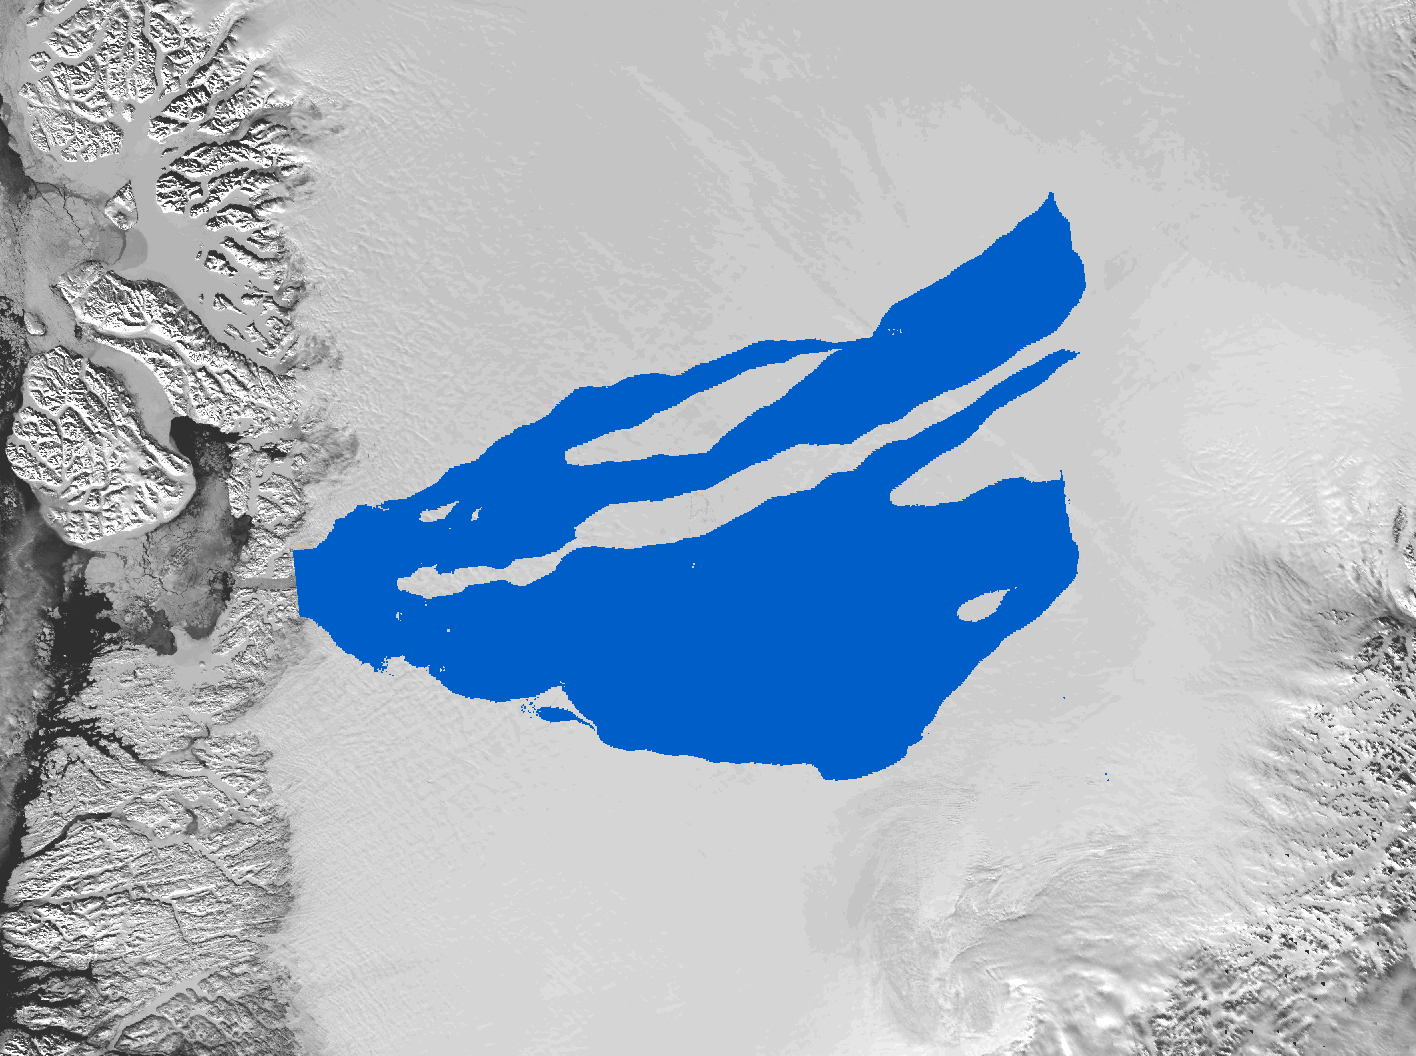
\includegraphics[width=0.85\textwidth]{hydro-mask}

basin for $-\nabla \phi$ flow,

where $\phi = \rho_i g H + \rho_w g b$,

for subglacial water
\end{center}
\end{column}
\end{columns}

\end{frame}


\setbeamertemplate{background canvas}
{
  \tikz{\node[inner sep=0pt,opacity=0.3] {\includegraphics[width=\paperwidth]{crop-andy-66}};}
} 


\begin{frame}
  \frametitle{summary}

  \begin{itemize}
  \item we will put the ``basic'' model in PISM
    \begin{itemize}
    \small
    \item[$\ast$] mass conservation
    \item[$\ast$] numerical stability provable for low-order scheme
    \item[$\ast$] allows (needs?) over-regularization
    \item[$\ast$] degree of coupling to sliding: needs exploration
    \end{itemize}
    \normalsize
  \item next: extend basic model to more dynamic subglacial drainage systems
    \begin{itemize}
    \small
    \item[$\ast$] nontrivial job: wall melt and channelization (\emph{as we all know})
    \item[$\ast$] the 2D spatial averages must be captured
    \end{itemize}
    \normalsize
  \item we are aware of the danger of building a model whose parameters cannot be identified
    \begin{itemize}
    \small
    \item[$\ast$] too much depends on surface observations of flow
    \end{itemize}
    \normalsize
  \end{itemize}

\vspace{17mm}
  \begin{center}
  \tiny \emph{Thanks for help with figures: Andy Aschwanden, Sarah Child, Brad Gooch}
  \end{center}
\end{frame}








\end{document}
